\documentclass[a4paper, 11pt]{book}
\usepackage{graphicx}
\title{Python for the Under 10's}
\author{Graeme Winter}
\begin{document}
\maketitle
\clearpage
\thispagestyle{plain}
\par\vspace*{.35\textheight}{\centering For Emily, I hope you find
  this fun\par}
\chapter{Introduction}

\section{Preface for Grown Ups}

When the author was a child computers were smaller, simpler and harder to break\footnote{Machines like the BBC Model B, ZX81 and Spectrum 48k spring to mind}, and so much more suitable for leaning how they work. Today computers are bigger, more complex, easier to break and much less straightforward to understand. At the same time they are used for everything: from catching up on TV to reading the news, communicating with people and gaming. This has meant that the creative process of writing simple computer programs (typically games) has been lost in favour of easily accessed entertainment. While none of this is a bad thing, it has removed the opportunity to learn \emph{how they work}. The idea of this book is to provide this opportunity, using free tools and real programming languages. 

The pre-requisite for this is a relatively recent computer - anything bought since about 2005 or so, running Windows, Linux or Mac OS X should be fine. The only dependency is the installation of Python 2.7.3 or later from http://www.python.org. If you have an old laptop lying around which used to be useful and is no longer, this will probably be fine. If you're feeling really keen the Raspberry Pi may be for you (http://wwww.raspberrypi.org) as this is a little computer aimed at children learning about computers, which will plug into the TV in the same way as computers from the mid 1980's did, only much more powerful...

\section{Preface for Children}

Most grown ups use computers for a lot of the day, but most of them
have no idea how they work - the idea of this book is to help you
learn how they work and what they can do. Telling the computer what to
do is called programming, and there are lots of different languages
you can use to tell the computer what to do. This book is about one
called Python (yes, like the snake) which is good because it is one of
the easiest and also lets you do fun things straight away. 

In the book the pictures are called ``figures'' and you will find that
they are numbered - when you get to a bit where it says ``look at
Figure~1'' you will need to look around to find a picture with
``Figure~1'' under it - it will usually have a few words there which
explain the picture. Also, the way that the computer instructions are
written will look a bit different - they will be written \verb|like this| which means ``this is something to type in'' or ``what the Python
window'' should look like.

Some people say programming is hard, and sometimes it is, but the hardest bit is thinking about what you want the computer to do in little pieces - once you have done this getting the computer to do the work is easy. That's enough - let's get started!

\section{Getting Started}

The only thing that is needed is to install Python - which you can download from http://www.python.org. This is free but it is probably better if a grown up installs it. To use it you will need to do some typing in something called a terminal - on an Apple computer they look like Figure~\ref{figure-terminal}.

\begin{figure}
\label{figure-terminal}
\centering
\fbox{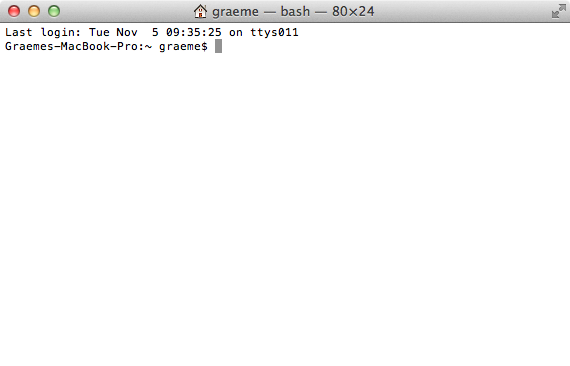
\includegraphics[scale=0.4]{terminal.png}}
\caption{The ``Terminal'' on an Apple computer - on a Windows computer
  this will look a little different.}
\end{figure}

\noindent
and they let you talk to the computer. All you need to do in here is type ``python'' and you should see

{\small
\begin{verbatim}
Python 2.7.3 (default_cci, Dec 13 2012, 05:32:36) 
[GCC 4.2.1 (Apple Inc. build 5666) (dot 3)] on darwin
Type "help", "copyright", "credits" or "license" for more information.
>>> 
\end{verbatim}
}

\noindent 
or something similar which says that the computer is ready to start talking to you in Python. If you see this then everything is set up just fine.

\chapter{Pythons and Turtles}

\section{Introduction}

Most programming books begin with showing how to print something (which means show it on the screen) usually ``Hello, World!'', and then move on to how to print your name, numbers and so on. This is not very interesting so this book will start with how to draw some shapes, which is a good way of learning how to tell the computer things, as you need to think hard about what you want first. For this we will use the Python turtle.

\section{The Python Turtle}

The Python turtle module (a module is a ``lump'' of computer program) is a little arrow which you can use to draw pictures. Unlike most drawing programs where you use a mouse to do drawing for this you need to tell it where to go. The simplest way to use it is to tell it to go forwards, backwards, left and right by certain amounts, and to lift the pen up and to put it down again. When you start it is pointing sideways.

This is where you need to start thinking about \emph{exactly} what you want the computer (or turtle) to do. Let's start by drawing a square. Easy right? But you need to imagine that you are walking around and holding a giant pen and blindfolded - how would you draw a square then? This is the kind of instructions you need to give the computer:

\begin{enumerate}
\item{Step forwards 100 paces}
\item{Turn left}
\item{Step forwards 100 paces}
\item{Turn left}
\item{Step forwards 100 paces}
\item{Turn left}
\item{Step forwards 100 paces}
\item{Turn left}
\end{enumerate}

\noindent
if you do this you should find you have drawn a square about 100 paces to a side. We really need to be more specific though - how far left to turn? Also it's boring to repeat yourself like this, but we will come back to that later with something called \emph{loops}. 

Here's some Python code to do exactly this:

{\small
\begin{verbatim}
import turtle
turtle.forward(100)
turtle.left(90)
turtle.forward(100)
turtle.left(90)
turtle.forward(100)
turtle.left(90)
turtle.forward(100)
turtle.left(90)
\end{verbatim}
}

\noindent
If you type this into the Python window you should see a new white
square window pop up and a little white box will appear like
Figure~\ref{figure-turtle-001-square} and your Python window should looks like this:

{\small
\begin{verbatim}
Graemes-MacBook-Pro:~ graeme$ python
Python 2.7.1 (r271:86832, Jul 31 2011, 19:30:53) 
[GCC 4.2.1 (Based on Apple Inc. build 5658) (LLVM build 2335.15.00)] on darwin
Type "help", "copyright", "credits" or "license" for more information.
>>> import turtle
>>> turtle.forward(100)
>>> turtle.left(90)
>>> turtle.forward(100)
>>> turtle.left(90)
>>> turtle.forward(100)
>>> turtle.left(90)
>>> turtle.forward(100)
>>> turtle.left(90)
>>> 
\end{verbatim}
}

\begin{figure}
\label{figure-turtle-001-square}
\centering
\fbox{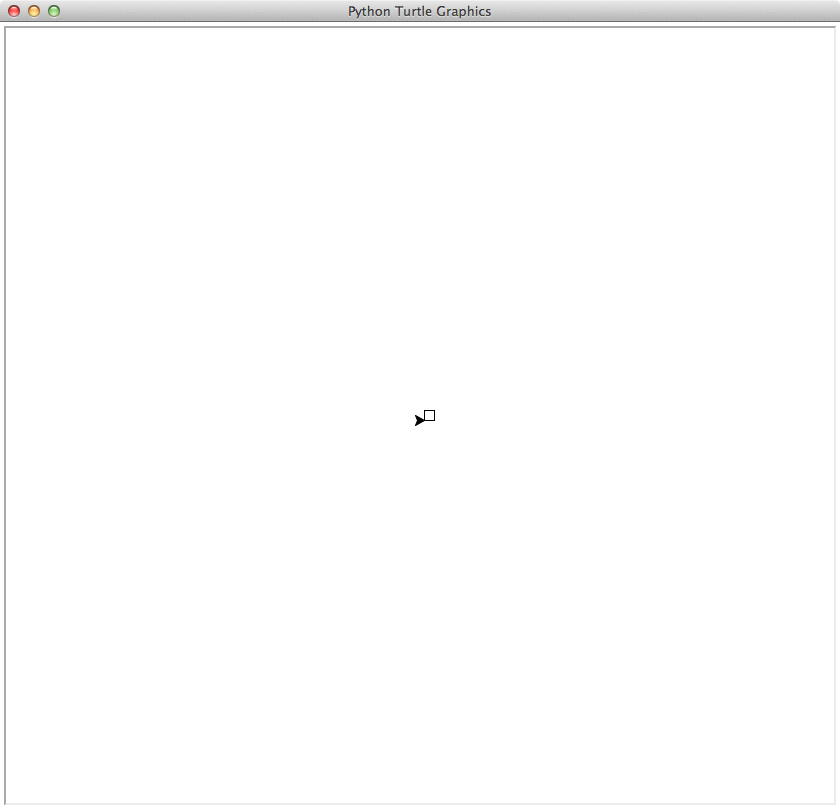
\includegraphics[scale=0.4]{turtle-001-square.png}}
\caption{The square drawn by the turtle after stepping forward 100 and
  turning left 90 four times.}
\end{figure}

What we have done here is to say first "I would like to use the turtle" then we have said four times to move forward 100 steps and to turn left by 90 degrees (which is a corner on a square.) You may find after you have typed all of this that you did not need to type it all, as Python remembers what you have done and so you can sometimes just press the "up" arrow on the keyboard and re-run some of the things you have typed already.

You can also lift the pen up with \verb|turtle.penup()| and put it down again with \verb|turtle.pendown()| - with these it is possible to draw some very fancy pictures limited only by your imagination and patience! Why not go and play some. When you've drawn some pictures ``by hand'' like this let's find out about loops.

\section{Loops}

Just to draw a square earlier took a lot of typing - when you are a computer it can take a lot of instructions to do something simple. There are easier ways to do this though, and one of them is to have something called a loop. Loops are easy - they just say to do the same thing over and over again. We could draw the square with a loop like this:

{\small
\begin{verbatim}
import turtle
for j in range(4):
  turtle.forward(100)
  turtle.left(90)
\end{verbatim}
}

\noindent 
which tells the computer to do the same thing four times. It is useful to look at these lines one at a time. If you type \verb|range(4)| you will see \verb|[0, 1, 2, 3]| - this is what Python calls a list, and it is a list of numbers which go from 0 to 3. This is Python's way of counting which is a bit odd but you will get used to it. Then we have the \verb|turtle.forward(100)| command and the \verb|turtle.left(90)| command a little way in - there are two spaces in front. This says that these instructions are \emph{inside} the loop. If you do this you will find it draws exactly the same square as earlier. You can also have something like:

{\small
\begin{verbatim}
for j in range(4):
  print j
\end{verbatim}
}

\noindent 
which will just print the numbers from 0 to 3 (counting again) like this:

{\small
\begin{verbatim}
>>> for j in range(4):
...   print j
... 
0
1
2
3
\end{verbatim}
}

\noindent
What is happening here is that \verb|j| is set to 0, then the print command is done, then \verb|j| is set to 1 and the print command is done and do on. When we draw a square we don't use the \verb|j| for anything, but when we print it we do. The fun thing about loops though is we can do things a lot more than four times - what do you think

{\small
\begin{verbatim}
import turtle
for j in range(360):
  turtle.forward(1)
  turtle.left(1)
\end{verbatim}
}

\noindent
will do? Why not type it in and find out? And be sure to get those
spaces right! Also what about:

{\small
\begin{verbatim}
import turtle
for j in range(60):
  turtle.forward(j)
  turtle.left(90)
\end{verbatim}
}

Finally all of these examples assume you have started from a new
Python - if you want to use one which is going already just use:

{\small
\begin{verbatim}
turtle.reset()
\end{verbatim}
}

\noindent
which clears the screen - you also don't need to keep typing import
turtle as after the first time you already have it.

\section{Mistakes}

Sometimes you will type things in wrong - this is fine and everyone does this - when you do make a mistake Python will complain that it does not understand, and usually this will have the word ``Error:'' in the message and it will try to explain what was wrong. When you have done this a lot you will find that these messages make sense but right now don't worry.

{\small
\begin{verbatim}
>>> import turtle
>>> for j in range(360):
...   turtle.forwards(1)
...   turtle.left(1)
... 
Traceback (most recent call last):
  File "<stdin>", line 2, in <module>
AttributeError: 'module' object has no attribute 'forwards'
\end{verbatim}
}

\chapter{Programming Python}

\section{Variables}



\end{document}
